\documentclass[../../main.tex]{subfiles}
%\usepackage{longtable}

\begin{document}

\begin{longtable}{| p{.20\textwidth} | p{.80\textwidth} |} 
\hline
    Kratak opis &  Administrator kreira novo takmičenje, unosi potrebne informacije i ukoliko želi šalje obaveštenje o takmičenju klijentima. Baza podataka se ažurira sa unetim informacijama.\\ 
\hline    
    Učesnici & Administrator - želi da kreira novo takmičenje u svojoj teretani.\\
\hline
   Preduslovi & Sistem je u funkciji i administrator je ulogovan na sistem. \\
\hline  
    Postuslovi & Kreirano je novo takmičenje i baza je ažurirana.\\
\hline
    Osnovni tok & \begin{enumerate}
        \item Administrator bira opciju u sistemu "Novo takmičenje".
        \item Administrator unosi potrebne informacije o takmičenju i pritiska dugme ''Zakaži takmičenje".
        \item Sistem proverava da li su podaci ispravni.
        \item Sistem nudi administratoru izbor kome želi da pošalje obaveštenje o takmičenju preko e-maila.
        \item Administrator bira kome da se pošalje obaveštenje o takmičenju i pritiska dugme "Pošalji obaveštenje".
        \item Sistem šalje obaveštenje i obaveštava administratora da su mejlovi poslati.
    \end{enumerate}\\
\hline
    Alternativni tokovi &  \begin{itemize}
        \item[A1] Pad sistema: Ukoliko u bilo kom koraku dođe do pada sistema administrator se ponovo loguje na sistem. Slučaj se nastavlja na koraku 1.  
        \item[A3] Neispravni podaci: Sistem obaveštava koja polja nisu ispravno popunjena. Slučaj se nastavlja na koraku 2.
    \end{itemize}\\
\hline
    Podtokovi & /\\
\hline
    Specijalni zahtevi & /\\
\hline
    Dodatne informacije & \begin{enumerate}
        \item Informacije koje sistem traži za zakazivanje takmičenja: datum, vreme, lokacija, discipline, nagrade, participacija, sudije i dodatne informacije.
        \item Mogućnosti za slanje e-maila: trenerima i/ili klijentima.
    \end{enumerate}\\
\hline
\caption{Kreiranje novog takmičenja}
\end{longtable}

\begin{figure}[!ht]
\begin{center}
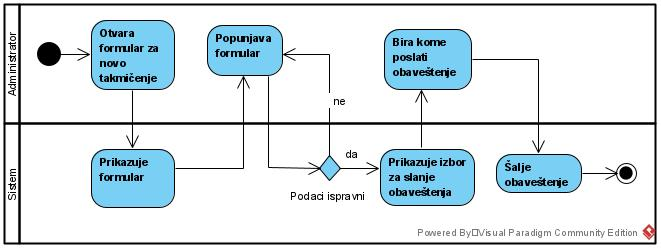
\includegraphics[scale=0.55]{sections/images/dijagram_atkivnovnosti_kreiranje_takmicenja.jpg}
\end{center}
\caption{Dijagram aktivnosti za kreiranje novog takmičenja}
\label{fig:kontekst}
\end{figure}

\end{document}